\documentclass[brazil]{beamer}
\usepackage{beamerthemesplit}
\usepackage[brazilian]{babel}
\usepackage[utf8]{inputenc}
\usepackage{hyperref}
\usepackage{color}
\usepackage{xcolor}
\usepackage{amssymb}
\usepackage{amsmath}
\usepackage{fancybox}
\usepackage{ulem}
\usepackage{listings}
\usetheme{Copenhagen}
\usecolortheme{seahorse}
\usefonttheme{serif}

% lembrete: \vspace{0.4cm}

\title{Can We Pay For What We Get In 3G Data Access?}
\author{Diogo Haruki Kykuta}
\date{}

\begin{document}

\frame{\titlepage}

%-------------------------------------
% INTRODUÇÃO
%-------------------------------------
\section{Introdução}


\frame{\begin{center}
        \Huge Introdução
\end{center}}

\subsection{Motivação}

\begin{frame}[fragile]
    \frametitle{Motivação}
    \begin{itemize}
        \item Experiências ruins com 3G
        \item Queda de velocidade no final do mês, mesmo eu achando que estava abaixo do "limite"
    \end{itemize}
\end{frame}

\begin{frame}[fragile]
    De acordo com a operadora, posso navegar até 300MB no mês usando até 1Mbps, após isso, a velocidade cai
    para 50 kbps.

    \pause
    \vspace{0.4cm}
    Mas eu já experimentei essa diminuição de velocidade mesmo não tendo atingido o limite.
\end{frame}

\begin{frame}[fragile]
    \frametitle{Cenário}
    Um exemplo: Alice só se lembra de ter baixado um aplicativo de 2MB da App Store.

    \begin{figure}
    \begin{center}
        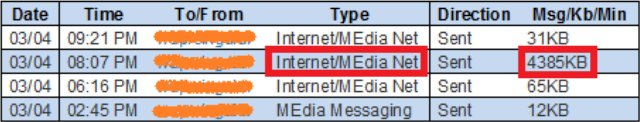
\includegraphics[scale=0.5]{images/contaAlice.jpg}
    \end{center}
    \end{figure}
\end{frame}

\subsection{O paper}
\begin{frame}[fragile]
    \frametitle{O paper}
    \begin{center}
        Chunyi Peng, Guan-Hua Tu, Chi-Yu Li, Songwu Lu
    \end{center}
    \vspace{0.4cm}
    \begin{itemize}
        \item Estudo em casos normais e extremos.
        \item UDP e TCP.
        \item Navegar sem serem cobrados.

    \end{itemize}
\end{frame}

\subsection{Os testes}
\begin{frame}[fragile]
    Os testes foram feitos usando duas grandes operadoras dos EUA. \\
    Com algumas comparações (em certos casos) com uma terceira operadora e com operadoras chinesas.
\end{frame}

\begin{frame}
    \begin{figure}
    \begin{center}
        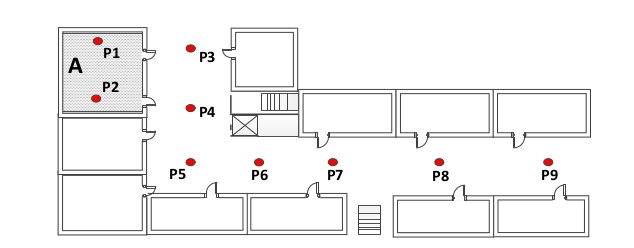
\includegraphics[scale=0.3]{images/sala.jpg}
    \end{center}
    \end{figure}
\end{frame}


\section{Casos Extremos}
\frame{\begin{center}
        \Huge Casos Extremos
\end{center}}

\subsection{UDP sem controle}

\begin{frame}[fragile]
    UDP não tem verificação de recebimento de pacote. \\
    A operadora recebe os pacotes do servidor, mas não consegue mandar para o dispositivo móvel. Mas ainda assim, são cobrados.
\end{frame}

\begin{frame}[fragile]
    O que importa é a quantidade de pacotes que chega na operadora, e não quantos pacotes chegam na Unidade Móvel.
\end{frame}

\subsection{Velocidade maior do que a compatível}

\begin{frame}[fragile]
    TCP tem controle de fluxo, portanto, pacotes não recebidos não devolvem ACK. Assim, não são tantos pacotes perdidos e a diferença não é tão grande.
    
\end{frame}

\begin{frame}[fragile]
    UDP não tem. Portanto os pacotes entram na operadora com a velocidade enviada pelo servidor e são armazenadas em um buffer para serem enviadas conforme for possível. 

    \vspace{0.3cm}
    Mas esse buffer tem tamanho limitado $\rightarrow$ perda de pacotes.
\end{frame}

\section{Casos Normais}

\frame{\begin{center}
        \Huge Casos Normais
\end{center}}

% Páginas 7 e 8

\begin{frame}[fragile]
% Aqui eu preciso da imagem do começo
        \frametitle{Quick Fix}
        \begin{itemize}
            \item Feedback do RNC sobre pacotes não enviaddos para a U.M.
            \item Timer para interromper a tentativa de enviar dados quando não tem sinal
            \item Big Data $\rightarrow$ a rede deve verificar a situação do dispositivo
        \end{itemize}
\end{frame}

\section{Gray Areas}
\frame{\begin{center}
        \Huge Gray Areas
\end{center}}

\subsection{Envio de dados para IP errado}

\begin{frame}[fragile]
    Enviar dados via UDP para um IP inválido gera cobrança.

    \vspace{0.4cm}
    Por TCP, em pouco tempo o envio é interrompido, pela ausência de ACKs.
\end{frame}

\begin{frame}[fragile]
    \frametitle{Middleboxes}
    Proxy servers, CDN servers, NAT boxes, firewalls

    \vspace{0.4cm}
    \pause
    Em uma das operadoras testadas, existia alguma middlebox, fazendo com que a unidade móvel recebesse os ACKs, portanto a conexão não era interrompida como deveria.
\end{frame}

\subsection{Outras aplicações}

\begin{frame}[fragile]
    \frametitle{FTP}
    FTP usa duas sessões TCP: uma na porta 21 (comandos) e uma na porta 20 (tranferência de dados).

    \vspace{0.5cm}
    Ambas são cobradas.
\end{frame}

\begin{frame}[fragile]
    \frametitle{Links quebrados}
    O resultado final é o aviso do erro, mas ainda assim a transmissão desses dados é cobrada.

    E em quantidade diferente.

    \begin{figure}
    \begin{center}
        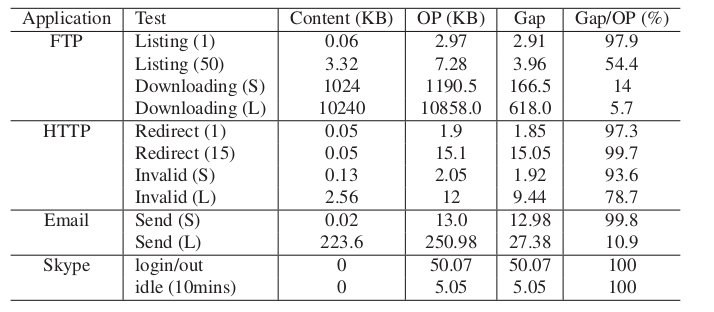
\includegraphics[scale=0.3]{images/applications.jpg}
    \end{center}
    \end{figure}
\end{frame}

\begin{frame}[fragile]
    \frametitle{Redirecionamentos}
    O usuário mal percebe o que acontece, mas acaba sendo cobrado pelos redirecionamentos. Até mesmo no caso de 15 redirecionamentos.
\end{frame}

\section{Driblando a cobrança}
\frame{\begin{center}
        \Huge Driblando a cobrança
\end{center}}

\subsection{DNS não cobrado}
\begin{frame}[fragile]
    Serviço de DNS: porta 53.

    \vspace{0.4cm}
    \Huge{Não é cobrado}
\end{frame}



\end{document}
